\chapter{Modeling process}
\label{ch:MP}

\section{Data Preparation}
\label{sec:dataprep}
Explanatory factors can be split into numerical, categorical and indicator variables. Within the corporate segment, these risk factors mostly take the form of numerical variables, such as financial ratios and macroeconomic conditions. The retail sector typically involves categorical factors, including profession, marital status and residential status. Even numerical values like age or employment duration often undergo a binning process, transforming them into categories (e.g., "20-25 years," "25-30 years"). If a categorical variable assumes too many distinct values or one category comprises a minimal proportion of observations (adhering to a rule of thumb of at least 5\% per bucket), merging categories might be beneficial.

One effective approach is consolidating categories with similar default rates or utilizing measures like \ac{WoE} and \ac{IV}, as Equations \ref{dp_woe} and \ref{dp_iv} outlined. WoE measures the discriminatory power of each risk factor value - a positive WoE means a relatively low risk and a negative Woe indicates a relatively high risk. Meanwhile, IV assesses the whole variable's capability to distinguish between default and non-default events; a higher IV corresponds to better discriminatory power and vice versa.

As a final step, categorical variables must be transformed into dummy variables for the modeling process. In this context, if a variable encompasses n distinct values, n-1 dummy variables are generated. Omitting one dummy variable is crucial to prevent the introduction of a linear combination during the modeling process, as illustrated in Figure \ref{fig:dp_dumenc} and indicated by the crossed-out column. \footnote{\cite{Witzany:2017} pp.~47-51}

\begin{equation}
\text{WoE} = \ln\left(\frac{\text{Distribution of Non-Default}}{\text{Distribution of Default}}\right) \label{dp_woe}
\end{equation}
\begin{equation}
\text{IV} = \sum_{i=1}^{n} (\text{Distribution of Non-Default} - \text{Distribution of Default}) \times WoE \label{dp_iv}
\end{equation}
where:
\begin{conditions}
n  	& number of categories or buckets 
\end{conditions}

\begin{figure}[H]
	\centering
	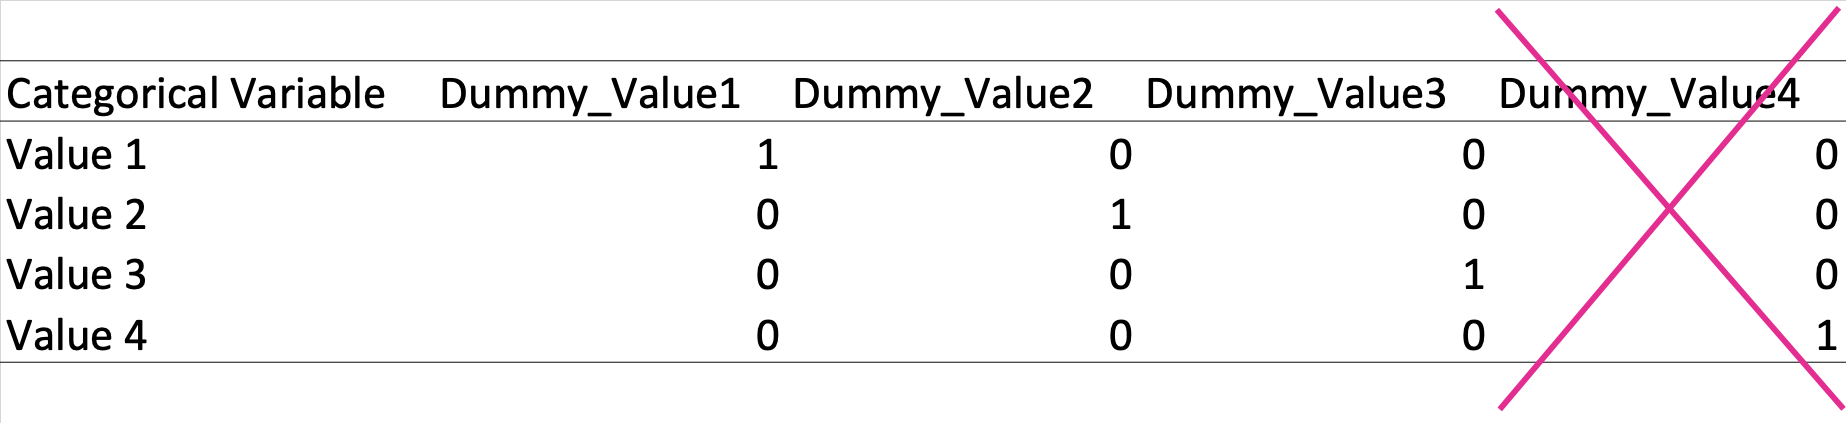
\includegraphics[width=0.625\textwidth]{./MP__encoding.png}
    \caption{Dummy encoding, Omission of one dummy column}
    \label{fig:dp_dumenc}
\end{figure}

\subsection{Missing Data Handling}
A common problem in real data sets is missing information, which needs to be appropriately handled during the modeling process. Popular approaches involve replacing missing values through statistical methods such as mean and median or algorithm-based imputation, such as the k-nearest neighbor Imputer. In the latter case,  the missing value gets imputed with the average value of its k-nearest neighbors, a process detailed in Chapter \ref{sec:kNN}. While another option is to eliminate data entries with missing information, this approach comes with potential drawbacks like information loss and bias. In the case of categorical variables, an alternative method is to treat missing information as a distinct category labeled "Missing", which removes the need for additional adaptations.~\footnote{\cite{Python:2022} p.~207}

\subsection{Erroneous Data Handling}
Erroneous data originating from data entry mistakes or inconsistencies have the potential to introduce noise and bias into the PD modeling process. Expert knowledge is crucial in identifying and rectifying such erroneous data. The best way to reduce incorrect data is control procedures implemented in the data entry systems and a data quality framework, where data validation rules are applied to identify inconsistent or illogical data. These data entries can be treated as missing information for the data preparation process.


\subsection{Outlier Detection and Treatment}
\label{sec:OutlTr}
Extreme values, also called Outliers, can significantly impact the estimated PD model, making expert knowledge crucial in this domain as well. Variables resulting from ratio calculations are especially sensible to outliers, particularly when dealing with division by small numbers. Visual inspection is a simple technique for outlier detection, but this would become impractical with the increasing number of variables. To address this, quantitative approaches become invaluable, utilizing statistical measures such as \ac{IQR}, box plots or Z-scores to identify outliers. A boxplot, also known as a box-and-whisker plot, is a visual representation of the variable's distribution and spread, with the box representing the \ac{IQR} and the whiskers denoting the upper and lower limits. An example is displayed in Figure \ref{fig:dp_iqr_boxpl}. The Z-Score, on the other hand, shows how many standard deviations a data point deviates from the mean of a data set. After the detection, a popular method to treat outliers is winsorization, where all values above or below a certain threshold are capped to the upper and lower limit, thereby minimizing the impact of outliers on the PD model.\footnote{\cite{Python:2022} p.~250}

\begin{figure}[H]
\begin{minipage}{.5\textwidth}
	\begin{align} 
	IQR &= Q_3 - Q_1 \label{eq:dp_iqr_boxpl1}\\
	Upper Limit &= Q_3 + 1.5 \times IQR \label{eq:dp_iqr_boxpl2}\\
	Lower Limit &= Q_1 - 1.5 \times IQR \label{eq:dp_iqr_boxpl3}
	\end{align}
	where:
	\begin{conditions}
	Q_{3}  		& 3.Quartile \\
	Q_{1}  		& 1.Quartile \\
	\end{conditions}
\end{minipage}%
\begin{minipage}{.5\textwidth}
	\centering
	\includegraphics[width=0.9\textwidth]{./MP__boxplot.png}
\end{minipage}
    \caption{Interquartile range and boxplot, Source: \cite{Boxplot:2019}}
    \label{fig:dp_iqr_boxpl}
\end{figure}

\section{Modeling process: Logistic Regression}

\subsection{Variable selection}
During the modeling process, the aim is to estimate a model that shows the best performance within an in-sample and within an out-sample data set. An approach incorporating all available information into the scoring function may indeed yield a high discriminatory power within the trained sample. However, this method usually results in multiple variables exhibiting insignificant coefficients: their p-values fall below the designated confidence level, making it impossible to reject the null hypothesis asserting that the coefficient is, in fact, zero. This outcome not only widens the confidence level but also raises concerns about the accuracy of the coefficient's sign. Therefore, the model's performance on a different data set, especially on more recent data, will most likely deteriorate, leading to unstable predictions. To address this challenge, an extensive analysis of variable performance, considerate selection processes and expert knowledge become crucial.\footnote{\cite{Witzany:2017} p.~44}

\subsubsection{Univariate Analysis}
As a first step, all available variables should be considered for the modeling process. Then, an assessment of the missing rate, detection of outliers and the plausibility of values is conducted. If the variable complies with all data quality requirements, its discriminatory power is then evaluated. This evaluation can be executed using either the univariate Gini coefficient or Information Value. Detailed explanations for both measures are provided in Chapters \ref{sec:gini} and \ref{sec:dataprep}, respectively. The remaining risk factors exhibiting satisfactory discriminatory power form the basis of the long list. 

\subsubsection{Multivariate Analysis}
Maintaining a low level of correlation among model variables is essential to avoid issues related to multicollinearity, which can lead to unstable coefficient estimates in the modeling process. The correlation between two variables can be measured using the Pearson or Spearman correlation coefficient, as detailed in Equations \ref{eq:dp_pears} and \ref{eq:dp_spear}. The Pearson correlation coefficient is more appropriate if a linear relationship is present, while the Spearman correlation coefficient excels in detecting non-linear interactions and can even be used for ordinal variables. The coefficient ranges from -1 (perfect negative correlation) to 1 (perfect positive correlation), with 0 indicating no correlation.\footnote{\cite{FUMS:2020} pp.~129-131}

After computing the coefficients for each variable pair, all values can be arranged into a correlation matrix. An example is visible in Figure \ref{fig:dp_corrmatrix}, which is the heatmap version of Table \ref{tab:re_corr_matrix}. If two variables are highly correlated with a correlation coefficient above a pre-defined threshold, the variable with the lower discriminatory power should be removed from the model list. 

\begin{equation}
\hat{\rho} = \frac{\sum_{i=1}^{n} (x_i - \hat{y}_X)(y_i - \hat{y}_Y)}{\sqrt{\sum_{i=1}^{n} (x_i - \hat{x}_X)^2 \sum_{i=1}^{n} (y_i - \hat{y}_Y)}} \label{eq:dp_pears}
\end{equation}
where:
\begin{conditions}
 x_i, y_i     				& individual observations \\
 \hat{y}_X, \hat{y}_Y    	& sample mean of X and Y  \\
 n    						& number of paired observations
\end{conditions}

\begin{equation}
\rho_s = 1 - \frac{6 \times \sum d_i^2}{n \times (n^2 - 1)} \label{eq:dp_spear}
\end{equation}
where:
\begin{conditions}
 d_{i}  & difference between the ranks of corresponding observations \\
 n    	& number of paired observations
\end{conditions}

\begin{figure}[H]
	\centering
	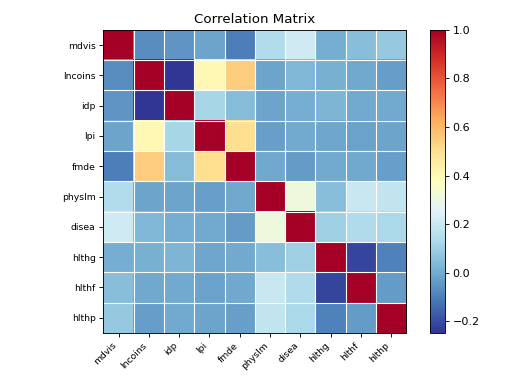
\includegraphics[width=0.625\textwidth]{./MP__corrmatrix.png}
    \caption{Correlation matrix example}
    \label{fig:dp_corrmatrix}
\end{figure}

In the case of categorical variables, the Variance Inflation Factor (VIF, Equation \ref{eq:dp_vif}), which measures the collinearity in the regression analysis, can be utilised. As a final refinement, adjustments based on expert judgment should be applied, allowing disqualified variables into the list or removing variables, even if they meet all criteria. Particular attention should be given to analyzing the relationship between explanatory factors and default rates. If the observed behavior contradicts economic rationale, the variable should be excluded from the model list, also known as the shortlist.\footnote{\cite{Witzany:2017} pp.~45, 53}


\begin{equation}
\text{VIF}_{i} = \frac{1}{1 - R_{i}^2} \label{eq:dp_vif}
\end{equation}
where:
\begin{conditions*}
 R_{i}^2  & coefficient of determination obtained by regressing the i-th regressor on all the other regressors
\end{conditions*}

\subsection{Modeling steps}
Upon identifying the  most promising key factors, there are different approaches to determine the final model variables, specifically, the forward, backward, forward stepwise and backward stepwise selection procedure. The forward approach starts with an empty model and step by step, the variable with the highest discriminatory power is incorporated contingent upon the significance of its coefficient (p-value below a specified threshold). This process continues until no variable satisfies the condition.

Conversely, in the backward selection procedure, the model starts with all variables and those are iteratively removed one by one based on the p-values of their coefficients, until only significant coefficients remain. The forward stepwise procedure combines elements of both with an initially empty model that progressively incorporates variables. However, after each addition, any variable losing significance will be removed. The backward stepwise procedure is the opposite process, starting with all variables and then eliminating those with non-significant coefficients. If, upon exclusion, any variables fulfill the significance condition once more, they are reintroduced into the model.\footnote{\cite{Witzany:2017} p.~45}

To attain a simple model incorporating only the most important risk drivers, the number of variables is limited utilizing the Akaike information criterion (AIC) and Bayesian information criterion (BIC). They are statistical measures used during model selection, which balances the goodness of fit of the model against the complexity by penalizing the inclusion of additional risk factors. At each step of the modeling process, the AIC and BIC are determined and the relative improvement per step is calculated. The model list is cut where a noticeable drop is detected, all subsequent variables are removed from the modeling process and the coefficients are re-estimated, resulting in the final model. 

\section{Modeling Process: Random Forest}

\subsection{Variable selection and Modeling steps}
\label{sec:mp_rf}
During the variable selection process of a normal decision tree, all available features are considered for a split. The evaluation involves assessing  the information gain or Gini impurity improvement for each value of a categorical or indicator variable, as well as for every possible split of a numerical risk factor. A split is executed for the maximum improvement and this process iterates for each resulting subsegment until a stopping condition is fulfilled. Variables that have already been used for a splitting condition maybe considered for a split again. Stopping conditions include achieving homogeneous subgroups, detecting no significant improvement, reaching the minimum leaf size, completing the maximum allowed splits or attaining the maximum depth of the tree.\footnote{\cite{BDT} pp.~2, 4}

As described in Chapter \ref{sec:dectrees}, a Random Forest model is built out of individually trained smaller decision trees and the prediction is a combination of the results of all decision trees, either by calculating the average or using the majority vote. During the training process, only a fraction of all possible features may be selected for the split and optionally, a fraction of the training sample can be used to prevent overfitting. This method is known as Bootstrap Aggregating or Bagging. These steps contribute to a more robust model by avoiding to rely on only a few specific features, which leads to a better generalization. The algorithm demonstrates reduced sensitivity to outliers, as individual decision trees may be affected, but the ensemble tends to mitigate their impact on the overall model. Missing values can still contribute to training the tree by considering other available features or may be randomly removed during the bagging process. A Random Forest model is also relatively robust compared to the logistic regression because, at each split, it selects a random subset of features and this helps in reducing the correlation between a set of features.\footnote{\cite{RanFor:2023}}

\subsection{Hyperparameter Tuning}
Hyperparameters are pre-set configurations of a machine learning algorithm, which are not trained but actually set prior to the training process. Examples are the number of neighbors for the kNN-algorithm, the count of layers in a neural network model or the number of trees in a Random Forest. An optimal configuration of the parameters is crucial because it directly impacts the model's performance to distinguish between the classes as well as influences overfitting. Adjusting these parameters is an individualized task, dependent on the unique characteristics of each problem, encompassing factors like the number and type of features, data size and data quality. With an increasing number of hyperparameters, the combination possibilities become extensive, making the search for the optimal configuration time-consuming. Therefore, the objective is to quickly identify a good configuration and subsequently search for potentially better settings.

Initially, a wide range of hyperparameter values is defined and the model's performance is assessed through randomly chosen combinations for a predefined number of iterations. The best combination is then utilized for the subsequent grid search. In this phase, a more constrained range for each hyperparameter, centered around the optimized configuration, is defined. All possible combinations within this scope are evaluated and the superior outcome from both approaches forms the final model configuration.\footnote{\cite{Python:2022} p.~465} \footnote{\cite{RanFor:2023}}

\subsection{k-Fold Cross Validation}
To further avoid overfitting, a cross-validation can be incorporated during the hyperparameter tuning process. The data set is randomly split into equally sized k subsamples, also called folds. The model with the tested hyperparameters is then trained on k-1 subsets and their performance is evaluated on the unused data set. This step is repeated k-times, with a different fold used for evaluation each time. The overall performance is calculated by averaging the metrics across all subsamples. This comprehensive process will be performed for each configuration setting during the random or grid search, contributing to a more robust model. An illustrative sketch is provided in Figure \ref{fig:re_wholesample}.\footnote{\cite{Python:2022} p.~470}

\begin{figure}[H]
	\centering
	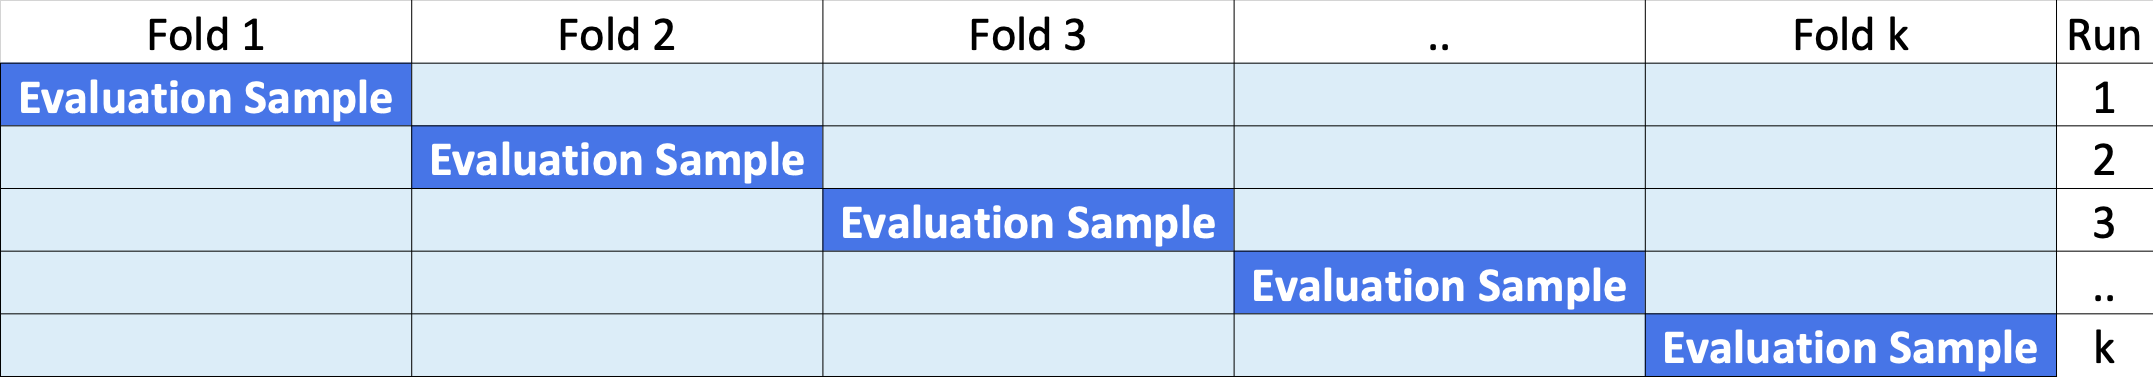
\includegraphics[width=0.65\textwidth]{./MP__kFold.png}
    \caption{k-Fold Cross Validation}
    \label{fig:re_wholesample}
\end{figure}